\section{Lezione 06 - 29/09/2023}
Continuiamo i nostri algoritmi sulle liste linkate
\subsection{Inserimento}
Andiamo a scrivere un algoritmo per l'inserimento in testa, cioè andiamo ad "attaccare" il nostro nuovo nodo all'inizio della lista, è il tipo di inserimento più semplice perché non prevede particolari modifiche alla struttura.
\paragraph{Funzione Ausiliaria} Useremo una funzione ausiliare per aiutarci in tutte le situazione di creazioni di un nuovo nodo:
\begin{lstlisting}[language=Java]
newNode(K,L) //K: Elemento, L:  Lista
	temp = allocanodo() //tipo una malloc
	temp->key = k //assegnamento valore
	temp->next = L //attacchiamo il nodo al primo elemento della lista in input
	return temp
\end{lstlisting}
Ora che abbiamo definito la nostra funzione ausiliaria andiamo a scrivere l'algoritmo di inserimento
\begin{lstlisting}[language=Java]
Insert(L,K)
	ret = search(L,K) //cerchiamo il valore
	if ret=NIL then //se non e' presente lo inseriamo
		L=newNode(K,L)
	return L
\end{lstlisting}

\subsection{Inserimento Ordinato (iterativo)}
Per strutturare al meglio le liste possiamo prevedere un inserimento ordinato, fare questo nelle liste è molto più efficiente rispetto a un array poiché non dobbiamo spostare tutti i valori per fare spazio al valore da inserire ma possiamo banalmente staccare i puntatori e "riattaccarli" nel modo corretto:
\begin{center}
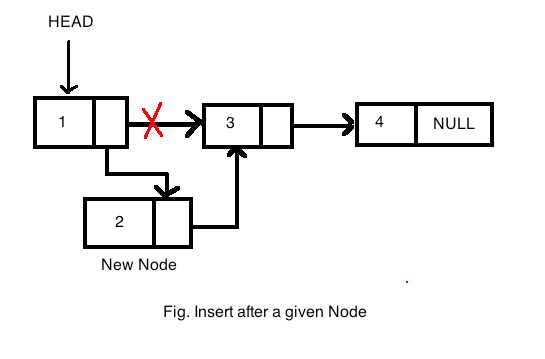
\includegraphics[width=0.6\textwidth]{insertAfterAGivenNode}
\end{center}
\newpage
Andiamo a definire l'algoritmo in maniera iterativa:
\begin{lstlisting}[language=Java]
InsertO(L,K)
	temp=L //salviamo il puntatore al primo elemento
	P=NIL //creiamo una variabile di appoggio
	while [temp != NIL and temp->key < k] do 
		P=temp //mettiamo P sul nodo "precedente" a dove inseriamo
		temp=temp->next //mettiamo temp sul nodo "successivo"
		
	if [temp = NIL or temp->key > k] then
		new=newNode(k,temp) //creiamo il nodo attaccandolo al "successivo"
		if P != NIL then //se "esiste" il precedente allora
			P->next = new //attacchiamo il "precedente" al nuovo
		else //se non esiste
			L=new //spostiamo la testa al nuovo valore 
			
	return L 	
\end{lstlisting}

\subsection{Inserimento Ordinato (ricorsivo)}
Come sempre per scrivere un buon algoritmo ricorsivo bisogna ragionare per casi, andiamo ad esaminare i vari possibili:
\begin{itemize}
\item Inserimento in testa (valore minimo)
\item Inserimento "centrale" (valore compreso tra due numeri)
\item Inserimento in coda (valore massimo)
\end{itemize}
Sulla base di ciò andiamo a scrivere il nostro algoritmo:
\begin{lstlisting}[language=Java]
InsertOR(L,K)
	if L=NIL then //Inserimento in coda
		L=newNode(K,L)
	else if [L->key > K] then //Inserimento in testa
		temp=L
		L=newNode(K, temp)
	else //Inserimento "centrale"
		L->next = InsertOR(L->next, K) //da esaminare
	return L 	
\end{lstlisting}

\subsection{Cancellazione (iterativa)}
Andiamo a scrivere un algoritmo di cancellazione simile a quello visto per l'inserimento, cioè andiamo a cercare il valore e ci posizioniamo sia "prima" che "dopo" il valore da cancellare.
\newpage
\begin{lstlisting}[language=Java]
Delete(L,K)
	temp=L //salviamo il puntatore al primo elemento
	P=NIL //creiamo una variabile di appoggio
	while [temp != NIL and temp->key != k] do 
		P=temp //mettiamo P sul nodo "precedente" a quello da cancellare
		temp=temp->next //mettiamo temp sul nodo da cancellare
		
	if temp != NIL then 
		if P != NIL then 
			P->next=temp->next
		else
			temp=L
			L=L->next
		dealloca(temp)
	return L 	
\end{lstlisting}

\subsection{Cancellazione (ricorsiva)}
Ragioniamo per casi anche se in questo caso sono solo i due banali, cioè il valore è presente oppure no, nello specifico noi andiamo a considerare sempre la testa della lista che piano a piano a decrementarsi fino ad arrivare ad essere vuota
\begin{lstlisting}[language=Java]
Delete(L,K)
	if L!=NIL then //La lista ha almeno un valore
		if L->key=k then //elemento in testa
			temp=L
			L=L->next
			dealloca(temp)
		else //elemento non in testa, "spostiamo" la testa in avanti
			L->next = delete(L->next, k)
	return L
\end{lstlisting}

